\documentclass[border=8pt]{standalone}
\usepackage{tikz}
\usepackage{amsmath,amssymb}
\usetikzlibrary{arrows.meta, positioning, fit, backgrounds, calc, decorations.pathreplacing}

\definecolor{accent}{HTML}{1B4F72}
\definecolor{accentdeep}{HTML}{0E2F44}
\definecolor{accentmid}{HTML}{2E86C1}
\definecolor{accentlight}{HTML}{EBF5FB}
\definecolor{gold}{HTML}{D4AC0D}
\definecolor{goldlight}{HTML}{FFF8DC}
\definecolor{bordersoft}{HTML}{BDC3C7}
\definecolor{frozenblock}{HTML}{E8E8E8}
\definecolor{textmuted}{HTML}{888888}

\begin{document}
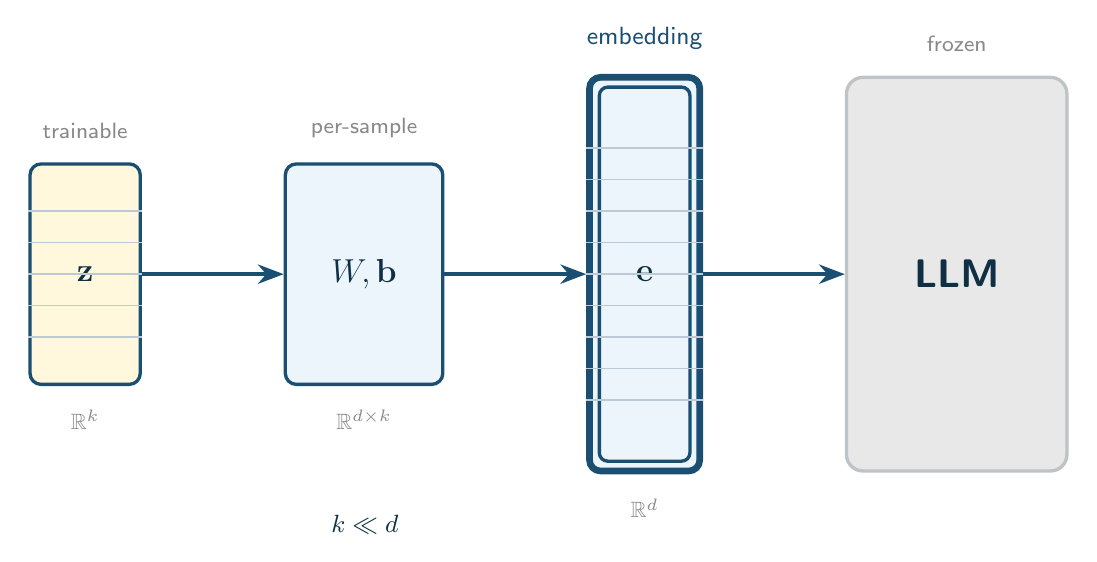
\begin{tikzpicture}[
    >=Stealth,
    font=\sffamily,
    every node/.style={inner sep=0pt},
    zvec/.style={
        draw=accent, line width=1.2pt, rounded corners=4pt,
        fill=goldlight, minimum width=14mm, minimum height=28mm,
        font=\sffamily\bfseries\large, text=accentdeep, align=center,
        inner sep=3pt
    },
    wmat/.style={
        draw=accent, line width=1.2pt, rounded corners=4pt,
        fill=accentlight, minimum width=20mm, minimum height=28mm,
        font=\sffamily\large, text=accentdeep, align=center,
        inner sep=3pt
    },
    evec/.style={
        draw=accent, line width=2.4pt, rounded corners=4pt,
        fill=accentlight, minimum width=14mm, minimum height=50mm,
        font=\sffamily\bfseries\large, text=accentdeep, align=center,
        inner sep=3pt
    },
    llmbox/.style={
        draw=bordersoft, line width=1.2pt, rounded corners=6pt,
        fill=frozenblock, minimum width=28mm, minimum height=50mm,
        font=\sffamily\bfseries\Large, text=accentdeep, align=center,
        inner sep=5pt
    },
    arrstyle/.style={->, line width=1.4pt, accent},
    label/.style={font=\sffamily\small, text=accent},
    mlabel/.style={font=\sffamily\footnotesize, text=textmuted},
]

% === z vector (low-dim) ===
\node[zvec] (z) {$\mathbf{z}$};
\node[mlabel, above=3mm of z] {trainable};
\node[mlabel, below=3mm of z] {$\mathbb{R}^k$};

% Draw z cells to show it's a small vector
\foreach \y in {-0.8, -0.4, 0, 0.4, 0.8} {
    \draw[accent!30, line width=0.5pt] ([yshift=\y cm]z.west) -- ([yshift=\y cm]z.east);
}

% === W matrix ===
\node[wmat, right=18mm of z] (W) {$W, \mathbf{b}$};
\node[mlabel, above=3mm of W] {per-sample};
\node[mlabel, below=3mm of W] {$\mathbb{R}^{d \times k}$};

% === e vector (full-dim) ===
\node[evec, right=18mm of W] (e) {$\mathbf{e}$};

% Draw double border on e (like the section 1 figure)
\node[draw=accent, line width=1.2pt, rounded corners=3pt,
      minimum width=11.5mm, minimum height=47.5mm,
      inner sep=0pt] at (e.center) {};

\node[label, above=3mm of e] {embedding};
\node[mlabel, below=3mm of e] {$\mathbb{R}^d$};

% Draw e cells to show it's a bigger vector
\foreach \y in {-1.6, -1.2, -0.8, -0.4, 0, 0.4, 0.8, 1.2, 1.6} {
    \draw[accent!30, line width=0.5pt] ([yshift=\y cm]e.west) -- ([yshift=\y cm]e.east);
}

% === Frozen LLM ===
\node[llmbox, right=18mm of e] (llm) {LLM};
\node[mlabel, above=3mm of llm] {frozen};

% === Arrows ===
\draw[arrstyle] (z.east) -- (W.west);
\draw[arrstyle] (W.east) -- (e.west);
\draw[arrstyle] (e.east) -- (llm.west);

% === k << d annotation ===
\node[font=\sffamily\small, text=accentdeep] at ($(z.south)!0.5!(e.south) + (0, -12mm)$) {$k \ll d$};

\end{tikzpicture}
\end{document}
